\documentclass[../ASSD_TP2.tex]{subfiles}
\begin{document}
\section{Espectrograma}

Un espectrograma es una imagen que muestra como varían a lo largo
del tiempo las frecuencias que componen a una señal dada. Para ello,
requiere aplicarle a la señal la transformada rápida de Fourier (FFT),
para luego realizar el mapeo. Para esta parte del trabajo, vamos a
explicar como funciona la función signal.spectrogram() de la librería
scypi.

\subsection{Parámetros que recibe}

La función nos da la posibilidad de recibir hasta 11 parámetros distintos,
aunque sólo el primero es obligatorio. Estos parámetros son: arreglo
con la señal, frecuencia de sampleo, ventana a utilizar por la FFT,
longitud de cada segmento, cantidad de elementos a repetir por cada
FFT (overlapping), longitud de la FFT, como desacoplar los valores,
dimensiones del arreglo de salida (haciendo referencia a si es un
numero complejo o flotante), escala (relacionado a las unidades de
los valores que se dibujan), ejes (escala de los ejes) y modo.

\subsection{Parámetros que devuelve}

La función devuelve el arreglo de frecuencias correspondiente, el
arreglo del tiempo correspondiente, y el arreglo con el espectro en
sí.

\subsection{Overlapping óptimo según el tipo de ventana}

Cuando la cantidad de datos es muy extensa en el tiempo, se suelen
dividir las muestras y aplicarle la FFT a cada una. Esto hace que
en determinados casos se pierda información de lo que sucede en el
tiempo y el espectro puede no representar fielmente a la señal en
su totalidad. Para evitar este efecto, se utiliza la técnica del overlapping,
la cual consiste en utilizar los últimos datos de una secuencia como
los primeros de la siguiente, de manera tal de que las FFT tengan
una mejor referencia temporal de lo que le ocurre a la señal en el
tiempo. 

Sin embargo, al haber distintos tipos de ventanas, existen distintos
valores de overlapping para cada una. A continuación se muestra una
tabla extraida del paper ``Spectrum and spectral density estimation
by the Discrete Fourier transform (DFT), including a comprehensive
list of window functions and some new flat-top windows.'' de G. Heinzel\textasteriskcentered ,
A. Ru\"{ }diger and R. Schilling, que detalla cual es el porcentaje
óptimo para cada tipo de ventana:

\begin{figure}[H]

\begin{centering}
\includegraphics[scale=0.6]{\string"imagenes/tabla\string".png}\caption{Parámetros de los distintos tipos de ventanas.}
\par\end{centering}
\end{figure}


\subsection{Espectrograma de una escala de Sol generado por ASDR}

Para este punto, se generó un archivo de sonido de una escala mayor
de Sol, para analizar luego con el espectrograma. La salida obtenida
fue la siguiente:

\begin{figure}[H]

\begin{centering}
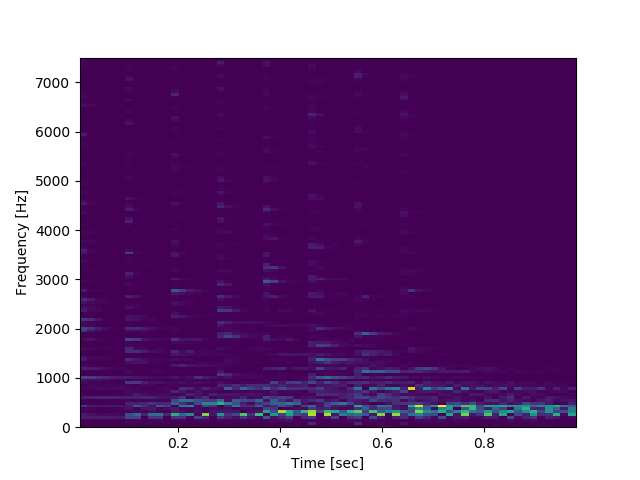
\includegraphics[scale=0.6]{imagenes/espectrograma}\caption{Espectrograma para una escala de Sol.}
\par\end{centering}
\end{figure}

Las frecuencias fundamentales de la escala fueron 196 Hz, 220Hz, 247Hz,
261Hz, 294Hz, 329Hz,370Hz y 392Hz pero vemos en el espectrograma que
las frecuencias presentes no son solo esas, sino que aparecen ténues
ruidos de frecuencias de hasta 7000Hz, haciendo énfasis en el rango
de 0 a 1000Hz en todo el tiempo. Ahora, si cambiamos los parámetros
de la FFT, junto con el overlapping, obtenemos los siguientes espectros:

\begin{figure}[H]

\centering{}\includegraphics[scale=0.55]{\string"imagenes/espect_overlap 25\string".png}\includegraphics[scale=0.55]{\string"imagenes/espect_overlap 50\string".png}\caption{Espectrogramas con overlapping de 25\% y 50\%.}
\end{figure}

Podemos ver que se pierde definición y fidelidad en ambos casos, aunque
se destaca que en la implementación con overlapping de 50\% el resultado
es mas fidedigno y no posee ruido.

\subsection{Conclusiones}

El espectrograma es una herramienta útil a la hora de analizar señales
y su espectro, pero debe utilizarse con sumo cuidado, puesto que posee
sus limitaciones. Para un uso óptimo, debe saberse el tipo de señal
que se desea analizar de antemano, para así de esta manera elegir
la ventana y su añcho más óptimos y con ellos su óptimo overlapping.
\end{document}
